\documentclass[11pt]{article}
\newcommand{\DoNotLoadEpstopdf}{}
\usepackage[T1]{fontenc}
\usepackage{lmodern}
\usepackage[margin=1.1in]{geometry}
\usepackage{amsmath,amssymb,amsthm}
\usepackage{microtype}
\usepackage{tikz}
\usepackage[hidelinks]{hyperref}
\input{glyphtounicode}
\input{glyphtounicode-cmex}
\pdfgentounicode=1
\pdftrailerid{}
\pdfsuppressptexinfo=15
\listfiles
\hypersetup{
  pdftitle={Uniform Permanence in Weakly Reversible Mass-Action Systems},
  pdfauthor={OpenAI},
  pdfsubject={Classwise permanence of weakly reversible reaction networks},
  pdfkeywords={mass-action systems, weak reversibility, permanence, affine approximation}
}
\newtheorem{theorem}{Theorem}[section]
\newtheorem{proposition}[theorem]{Proposition}
\newtheorem{lemma}[theorem]{Lemma}
\newtheorem{corollary}[theorem]{Corollary}
\theoremstyle{definition}
\newtheorem{definition}[theorem]{Definition}
\theoremstyle{remark}
\newtheorem{remark}[theorem]{Remark}
\newcommand{\R}{\mathbb R}
\newcommand{\Z}{\mathbb Z}
\newcommand{\norm}[1]{\left\|#1\right\|}
\newcommand{\abs}[1]{\left|#1\right|}
\newcommand{\one}{\mathbf 1}
\newcommand{\eps}{\varepsilon}
\DeclareMathOperator{\interior}{int}
\numberwithin{equation}{section}
\title{Uniform Permanence in\\Weakly Reversible Mass-Action Systems}
\author{OpenAI}
\date{October 5, 2026}
\begin{document}
\maketitle
\begin{abstract}
We prove the permanence conjecture for finite weakly reversible mass-action
systems with fixed positive reaction rates. Every positive stoichiometric
compatibility class admits one compact convex forward-invariant set that
every positive trajectory in that class enters in finite time, even when
the class is unbounded. The set depends only on the network, the rates, and
the class; the entry time may depend on the initial state. Thus, after its
entry time, every concentration satisfies the same positive lower and
finite upper bounds throughout that class.
\end{abstract}
\section{Introduction}\label{sec:introduction}

Weak reversibility requires every reaction in a chemical reaction network
to have a directed return path. It is natural to ask whether this graph
condition alone prevents concentrations from approaching zero or infinity.
Permanence asks for more: after a transient, all trajectories allowed by
the same conservation laws must satisfy the same positive lower and finite
upper bounds. We prove this conclusion for arbitrary finite weakly
reversible networks with fixed positive reaction rates.

\subsection{The problem and main result}

Let $d\geq1$. A finite reaction network consists of a set of
\emph{complexes} $C\subset\Z_{\geq0}^d$ and a set of directed
\emph{reactions} $R\subset C\times C$. We write $y\to y'$ for
$(y,y')\in R$. The network is \emph{weakly reversible} if for every
$y\to y'\in R$ there is a directed path from $y'$ to $y$. A
\emph{linkage class} is a connected component of the underlying undirected
graph. Assign a positive constant $k_{y\to y'}$ to each reaction. The
mass-action equation is
\begin{equation}\label{eq:mass-action}
  \dot x=f(x):=\sum_{y\to y'\in R} k_{y\to y'}x^y(y'-y),
  \qquad x^y:=\prod_{i=1}^d x_i^{y_i}.
\end{equation}
The \emph{stoichiometric subspace} and the \emph{positive stoichiometric
class} of $c\in\R_{>0}^d$ are
\[
  S:=\operatorname{span}_{\R}\{y'-y:y\to y'\in R\},
  \qquad P:=(c+S)\cap\R_{>0}^d.
\]
Since $f(x)\in S$, any positive solution starting in $P$ remains in $P$
for as long as it exists. The class $P$ need not be bounded.

A global positive trajectory is \emph{persistent} if
$\liminf_{t\to\infty}x_i(t)>0$ for every $i$. These lower bounds may
depend on the trajectory. We call the system \emph{permanent on $P$} if
every solution starting in $P$ is global and positive, and there is one
compact set $K\subset P$ that eventually contains each such solution.
The entry time may depend on the initial point, but $K$ may not. This is
the classwise uniformity in the permanence question
\cite[Definition~4.1]{BorosHofbauer2020}.

\begin{theorem}\label{thm:main}
Let $C\subset\Z_{\geq0}^d$ be finite, let $R\subset C\times C$ be
weakly reversible, and fix positive rate constants in
\eqref{eq:mass-action}. For every positive stoichiometric class $P$ there
is a nonempty compact convex set $K_P\subset P$ with the following
properties. Every initial point $x^0\in P$ gives a unique global positive
solution, and there is a finite $T(x^0)\geq0$ such that
\[
  x(t)\in K_P\qquad(t\geq T(x^0)).
\]
Moreover, $K_P$ is forward invariant. In particular, there is
$\eps_P\in(0,1)$, depending only on the network, the fixed rates, and
$P$, such that every such solution satisfies
\begin{equation}\label{eq:uniform-bounds}
  \eps_P\leq x_i(t)\leq\eps_P^{-1}
  \qquad(1\leq i\leq d,\ t\geq T(x^0)).
\end{equation}
\end{theorem}

Thus the fixed-positive-rate, weakly reversible formulation of the
permanence conjecture holds, including on unbounded classes. The
uniformity in \eqref{eq:uniform-bounds} is within each fixed class and
rate choice; the transient time is allowed to depend on $x^0$.

\subsection{Historical context and the contribution}

The structural theory of mass-action systems begins with the work of
Horn and Jackson and of Feinberg
\cite{HornJackson1972,Feinberg1972}. A system is \emph{complex-balanced}
if it has a positive state at which the total incoming and outgoing
reaction fluxes agree at each complex. For a complex-balanced system,
the classical theory gives a unique positive equilibrium in each
positive stoichiometric class and
an entropy-type Lyapunov function. Complex balance imposes conditions
on the rates as well as the graph; weak reversibility by itself does not
impose these balance identities. Feinberg's discussion of weakly
reversible systems \cite[Remark~6.1.E]{Feinberg1987} raised the question
of excluding limiting states with a zero concentration. Persistence
excludes approach to the boundary even along subsequences, and
permanence adds upper bounds and uniformity over initial points.

Important partial results developed both the dynamical picture and the
geometric methods. Anderson proved that every positive trajectory of a
complex-balanced system with one linkage class converges to its class's
positive equilibrium
\cite[Corollary~4.11]{Anderson2011}. Craciun, Nazarov, and Pantea proved
permanence for two-species weakly reversible systems, as part of their
more general theorem for endotactic networks
\cite[Theorem~6.4]{CraciunNazarovPantea2013}. Their endotactic condition
expresses an inward-pointing property of the reactions seen in every
direction. Pantea proved persistence of bounded
weakly reversible trajectories when $\dim S=2$, with no restriction to
two species \cite[Theorem~5.1]{Pantea2012}. Gopalkrishnan, Miller, and Shiu proved
permanence under the geometric condition of strong endotacticity,
which includes every weakly reversible network with one linkage class
\cite[Theorems~1.1 and~1.3]{GopalkrishnanMillerShiu2014}.
Boros and Hofbauer later gave another proof of the single-linkage
permanence theorem, producing a compact forward-invariant absorbing
set \cite[Theorem~4.2]{BorosHofbauer2020}. These permanence results
also permit rates varying in time within fixed positive bounds.

Craciun's toric-differential-inclusion approach constructs invariant
regions by comparing monomials in logarithmic coordinates. The revised
manuscript of September~23, 2026 proves persistence for bounded positive
trajectories of weakly reversible systems, including rates bounded above
and away from zero; its complex-balanced application establishes global
convergence \cite[Section~8, final remark]{Craciun2026}. The general
weakly reversible persistence statement there assumes boundedness of
the trajectory. Our theorem treats fixed rates and supplies one
eventual bound for every trajectory in a class.

The immediate input to the present argument is the affine approximation
lemma and trapping construction of \cite{OpenAI2026}. That paper proves
that every prescribed positive initial point belongs to a compact
convex forward-invariant set contained in the positive orthant. Such sets
give boundedness and persistence, but may depend on the initial point.
We reproduce the affine lemma and
its proof in Section~\ref{sec:affine}, and adapt the trapping construction
in Section~\ref{sec:trapping}. The additional arguments establish strict
increase away from a trapping set and connect trapping sets at different
scales. They turn bounds for individual trajectories into permanence
on a fixed class. Monomial comparisons and invariant regions have the
earlier antecedents just described; the affine approximation lemma is
credited to \cite[Lemma~2.1 and Corollary~2.2]{OpenAI2026}.

\subsection{Proof overview}

Fix one representative $c\in P$. For $0<h<1$, set
$B_h=[h,h^{-1}]^d$. Every $x\in B_h$ has a unique representation
$x=(h^{p_1},\ldots,h^{p_d})$ with $p\in[-1,1]^d$. The affine lemma
constructs a finite concave minimum
\[
  F_h(x)=\min_{\lambda\in\Lambda}
     \bigl(r_\lambda\cdot x+b_\lambda(h)\bigr),
\]
whose slopes $r_\lambda\in[-1,1]^d$ are independent of $h$. A label
$\lambda$ is \emph{active} at $x$ when it attains this minimum.
For any prescribed tolerance $E:[-1,1]^d\to(0,\infty)$, the construction
ensures
$\norm{r_\lambda-p}_\infty<E(r_\lambda)$ for every active label,
uniformly for small $h$. We choose the tolerance so that every nonzero
comparison $r_\lambda\cdot v$, where $v$ is a coordinate vector or a
difference of distinct complexes, has the same sign as $p\cdot v$.
To preserve these signs, our tolerance shrinks near a hyperplane
$r\cdot v=0$; on the hyperplane, the zero comparison imposes no
restriction. This is why the affine lemma allows a discontinuous
tolerance. When $r_\lambda\cdot v\ne0$, finiteness of the slope family
also gives a uniform positive lower bound for $\abs{p\cdot v}$.

At sufficiently small scales, the labels active at $c$ have zero slope,
so $F_h(c)$ is the global maximum of $F_h$. Its plateau
\[
  K_h:=\{x\in\R^d:F_h(x)=F_h(c)\}
\]
is compact and convex, contains $c$, and satisfies
$K_h\subset\operatorname{int}B_{\sqrt h}$
(Proposition~\ref{prop:plateau}). The restriction to $P$ now supplies
the decisive strictness condition. A member of the affine family whose slope lies
in $S^\perp$ is constant on $c+S$, so its value on $P$ is at least
$F_h(c)$. Such a label cannot be active at a point of $P\setminus K_h$.

For any active label $\lambda$, order the complexes by the levels
$r_\lambda\cdot y$, and separate consecutive levels by cuts. If a
downward reaction crosses a cut, its directed return path contains an
upward crossing. Monomials at lower source levels dominate those at
higher levels, so one upward flux exceeds the entire downward flux for
sufficiently small $h$. The net upward flux across each cut is therefore
nonnegative, and is positive whenever a reaction crosses it. Summing
these fluxes times the gaps between levels gives
$r_\lambda\cdot f(x)\geq0$, with strict inequality when
$r_\lambda\notin S^\perp$. Compactness at each fixed scale makes the
strict inequality uniform over all active labels to which it applies
(Proposition~\ref{prop:increase}). Thus $F_h$ is nondecreasing along
solution segments in $B_h$ and increases at a fixed positive rate on
$B_h\cap(P\setminus K_h)$. A trajectory in $P$ that stays in $B_h$
for all later times must reach $K_h$ in finite time and remain there.

Every initial point in $P$ belongs to some $K_h$, giving global
existence first. The inclusion $K_h\subset B_{\sqrt h}$ then permits
passage to a larger scale. Repeated square roots, capped at a scale
$h_P$ fixed by the class, reach $h_P$ after finitely many steps.
Section~\ref{sec:permanence} carries out this iteration and obtains
$K_P=K_{h_P}\cap(c+S)$, with $h_P$ chosen independently of the initial
point.

\section{Affine minima with arbitrary tolerance}
\label{sec:affine}

The proof will use a finite minimum of affine functions on the positive
orthant. Its essential property is that an active slope approximates the
exponent vector of the point where it is active. The allowed error will
depend on the slope and may be discontinuous. We prove the construction
and its uniform consequence from
\cite[Lemma~2.1 and Corollary~2.2]{OpenAI2026} in full.

For $m\geq1$, $u\in\R^m$, and $0<h<1$, put
\[
 X_h(u)=(h^{u_1},\ldots,h^{u_m}).
\]
A \emph{label} $\lambda=(r_\lambda,b_\lambda)$ consists of a slope
$r_\lambda\in\R^m$, independent of $h$, and an offset $b_\lambda(h)$
defined for all sufficiently small positive $h$. For a finite nonempty
family $\Lambda$ of labels, write
\[
 F_h(x)=\min_{\lambda\in\Lambda}
       \bigl(r_\lambda\cdot x+b_\lambda(h)\bigr).
\]
A label is \emph{active at $x$} if its affine value equals $F_h(x)$.
Every minimizing label is active when there is a tie. All offsets in a
finite family are understood to be restricted to a common interval on
which they are defined.

\begin{lemma}[Affine approximation with arbitrary tolerance]
\label{lem:affine}
Let $m\geq1$ be an integer, let $a<b$ be real numbers, and let
$E:[a,b]^m\to(0,\infty)$ be any function. There is a finite nonempty
family $\Lambda$ of labels with
\[
 r_\lambda\in[a,b]^m,
 \qquad b_\lambda(h)=o(h^a)\quad(h\to0+),
\]
such that the following implication holds. If $h_\nu\to0+$,
$p^\nu\in\R^m$ converges to $p\in[a,b]^m$, and a fixed label
$\lambda\in\Lambda$ is active at $X_{h_\nu}(p^\nu)$ for every $\nu$,
then
\[
 \norm{p-r_\lambda}_\infty<E(r_\lambda).
\]
The slopes and the family are independent of $h$. No regularity is
assumed of $E$, and the approximating vectors $p^\nu$ need not lie in
$[a,b]^m$.
\end{lemma}

\begin{proof}
We induct on $m$. Write $\mu(u)=\min_i u_i$ and
$\one=(1,\ldots,1)$. Since the largest coordinate of $X_h(u)$ is
$h^{\mu(u)}$, we first construct a family for each fixed value $t$ of
the smallest exponent. We then extend its guarantee to a neighborhood
of $t$ and combine finitely many such families by shifting their offsets.
The fixed-minimum construction is a singleton when $m=1$; the extension
and combination therefore also prove the base case.

Throughout the proof, asymptotic comparisons along $h_\nu\to0+$ and
$p^\nu\to p$ use fixed gaps between limiting exponents. In particular,
if $p_i>q$, then eventually $p_i^\nu\geq q+\delta$ for some
$\delta>0$, so $h_\nu^{p_i^\nu}=o(h_\nu^q)$; if $p_i<q$, the ratio
$h_\nu^{p_i^\nu}/h_\nu^q$ tends to infinity. We shall use these
comparisons only with strict limiting gaps.

\medskip
\noindent\emph{A family for a fixed minimum.}
Fix $t\in[a,b]$. We construct a finite family $\Lambda_t$ containing
$(t\one,0)$, with $\mu(r)=t$ for every slope, such that the conclusion
of the lemma holds for activity within $\Lambda_t$ whenever
$\mu(p)=t$.

If $m=1$ or $t=b$, the family $\{(t\one,0)\}$ suffices: a point
$p\in[a,b]^m$ with $\mu(p)=t$ then equals $t\one$. Otherwise
$m>1$ and $t<b$. Say a label has \emph{type $k$} if exactly $k$
entries of its slope exceed $t$, the remaining entries being $t$.
Start with the type~$0$ label $(t\one,0)$, and construct types
$k=1,\ldots,m-1$ successively. After type~$k-1$ has been constructed,
choose $\beta_k$ satisfying
\begin{gather*}
 t<\beta_k<b,\qquad
 \beta_k<\beta_{k-1}\quad\text{if }k>1,\\
 \beta_k-t<E(r)
 \quad\text{for every slope $r$ of type $k-1$.}
\end{gather*}
These conditions use only finitely many positive values of $E$, so
such a choice is possible. The new type~$k$ labels will force every
limiting exponent on a coordinate left at $t$ by a type~$k-1$ label
that stays active to be at most $\beta_k$. The last inequality will
then bound the error by that label's tolerance.

For each $k$-element coordinate set $U\subset\{1,\ldots,m\}$ and
$s\in[\beta_k,b]^U$, let $r(s)$ equal $s$ on $U$ and $t$ off $U$.
Apply the induction hypothesis in dimension $k$ to this cube with
tolerance $s\mapsto E(r(s))$, identifying $U$ with its naturally ordered
coordinates. For every resulting label $(s,d)$, add to $\Lambda_t$ the
type~$k$ label
\begin{equation}
 r=r(s),\qquad c(h)=-h^{\beta_k}+d(h),
 \qquad d(h)=o(h^{\beta_k}).
 \label{eq:local-labels}
\end{equation}
Here and below $c$ denotes a local offset. The resulting family is finite,
and all its offsets are $o(h^t)$. The negative offset favors raising
slope entries on coordinates where $X_h(p)$ is small; the decreasing
$\beta_k$ make that preference stronger with each successive type.

To verify the guarantee, let $p^\nu\to p\in[a,b]^m$ with
$\mu(p)=t$, and suppose a type~$k$ label $(r,c)$ stays active within
$\Lambda_t$ along $h_\nu\to0+$. Let $U$ be its raised coordinate set,
and abbreviate $h=h_\nu$. For $k>0$, comparison with $(t\one,0)$
gives
\[
 \sum_{i\in U}(r_i-t)h^{p_i^\nu}
 \leq h^{\beta_k}-d(h)=(1+o(1))h^{\beta_k}.
\]
Every coefficient on the left is at least $\beta_k-t>0$. A limiting
exponent $p_i<\beta_k$ would make the corresponding term divided by
$h^{\beta_k}$ tend to infinity. Therefore
\begin{equation}
 p_i\geq\beta_k\qquad(i\in U).
 \label{eq:raised-coordinates}
\end{equation}
Among labels made from this same $U$, all contributions off $U$ and
the term $-h^{\beta_k}$ are common. Thus $(s,d)$ is active in the
family furnished by induction. Its limiting exponent vector lies in
$[\beta_k,b]^U$, so
\[
 \max_{i\in U}\abs{p_i-r_i}<E(r).
\]
The approximating vectors $p_U^\nu$ may approach a face of that cube
from outside. This is why the induction statement allows them outside
the cube, including when $p_i=\beta_k$ or $p_i=b$.

It remains to bound the coordinates off $U$. This argument also includes
type~$0$, for which $U=\varnothing$. If $k<m-1$, we claim that
\[
 p_i\leq\beta_{k+1}\qquad(i\notin U).
\]
Otherwise choose $j\notin U$ with $p_j>\beta_{k+1}$ and any
type~$k+1$ label raised on $U\cup\{j\}$. Every limiting exponent
on this set exceeds $\beta_{k+1}$, by
\eqref{eq:raised-coordinates} and $\beta_k>\beta_{k+1}$ when
$k>0$. The competitor's affine value minus that of $(t\one,0)$ is
therefore
\[
 -h^{\beta_{k+1}}+o(h^{\beta_{k+1}}).
\]
For the supposed active label, the same difference is zero if $k=0$,
and is bounded below by $-h^{\beta_k}+o(h^{\beta_k})$ if $k>0$.
Since $h^{\beta_k}=o(h^{\beta_{k+1}})$, the competitor is strictly
smaller for all sufficiently small $h$ along the sequence, a
contradiction. Consequently, off $U$,
\[
 \abs{p_i-r_i}\leq\beta_{k+1}-t<E(r).
\]
If $k=m-1$, there is just one coordinate off $U$. Its limiting exponent
is $t$, since $\mu(p)=t$ and all coordinates on $U$ have limiting
exponents greater than $t$. Its error is zero. This proves the required
strict bound for every active label at the fixed minimum.

\medskip
\noindent\emph{Extension to nearby minima.}
For a fixed label $\lambda=(r,c)\in\Lambda_t$, let
$A_\lambda\subset[a,b]^m$ consist of the limits of all sequences
$p^\nu\in\R^m$ for which $h_\nu\to0+$ and $\lambda$ is active
within $\Lambda_t$ at $X_{h_\nu}(p^\nu)$. This set is closed.
Indeed, if $z_n\in A_\lambda$ and $z_n\to z$, choose from a
sequence realizing $z_n$ a parameter $0<h_n<1/n$ and a vector $u_n$
with $\norm{u_n-z_n}_\infty<1/n$ such that $\lambda$ is active at
$X_{h_n}(u_n)$.
Then $u_n\to z$, so this selected sequence realizes $z\in A_\lambda$.
This argument uses actual active points and requires no continuity of
the offsets in $h$.

The set of limits violating the desired estimate,
\[
 B_t=\bigcup_{\lambda=(r,c)\in\Lambda_t}
 \{p\in A_\lambda:\norm{p-r}_\infty\geq E(r)\},
\]
is compact: the union is finite and each $E(r)$ here is a fixed number.
The preceding argument shows that $B_t$ contains no point with
$\mu(p)=t$. Continuity of $\mu$ and compactness therefore give
$\rho_t>0$ such that $B_t$ contains no point with
\[
 \mu(p)\in I_t:=(t-\rho_t,t+\rho_t).
\]
If $B_t$ is empty any positive radius initially suffices; otherwise take
$\rho_t<\min_{p\in B_t}\abs{\mu(p)-t}$. Thus $\Lambda_t$
has the asserted limiting activity property whenever $\mu(p)\in I_t$.

Shrink $\rho_t$ further, if necessary, so that every local offset obeys
\begin{equation}
 c(h)=o(h^{t+\rho_t}).
 \label{eq:local-decay}
\end{equation}
For a nonsingleton family, choose $t+\rho_t<\min_k\beta_k$ and use
\eqref{eq:local-labels}; for a singleton the offset is zero.
We have obtained a family valid near each possible minimum exponent.
The remaining task is to ensure that a globally active label comes from
a family valid at its own limiting point.

\medskip
\noindent\emph{Combining the families.}
Take a finite subcover of $[a,b]$ from the intervals $I_t$. Discard
intervals contained in others, keeping just one if two coincide, and
order the remaining centers as $t_1<\cdots<t_N$. Write
$I_{t_j}=(L_j,R_j)$. Noncontainment forces both endpoints to have the
same strict order; since $t_j=(L_j+R_j)/2$, it is the order of the
centers. Hence
\[
 L_1<\cdots<L_N,\qquad R_1<\cdots<R_N.
\]
Consecutive intervals overlap. If $R_j\leq L_{j+1}$, a point of
$[R_j,L_{j+1}]\subset(t_j,t_{j+1})\subset[a,b]$ would be uncovered.
The first interval contains $a$ and the last contains $b$.

For $1\leq j<N$, choose a cut
\[
 q_j\in
 \bigl(\max\{t_j,L_{j+1}\},\min\{t_{j+1},R_j\}\bigr).
\]
The interval displayed is nonempty because consecutive intervals overlap
and each contains its own center. With $q_0=a$ and $q_N=b$, we have
\begin{equation}
 t_j<q_j<t_{j+1}\quad(1\leq j<N),
 \qquad [q_{j-1},q_j]\subset I_{t_j}\quad(1\leq j\leq N).
 \label{eq:affine-cuts}
\end{equation}
For $N=1$, the sole interval contains $[a,b]$ and no interior cuts are
needed. The closed intervals in \eqref{eq:affine-cuts} are the ranges
of minimum exponents assigned to the respective families; see
Figure~\ref{fig:intervals}.

Combine the selected families, replacing every local offset $c(h)$ in
$\Lambda_{t_j}$ by
\begin{equation}
 \widetilde c(h)=c(h)-\sum_{\ell=1}^{j-1}h^{q_\ell}.
 \label{eq:affine-shifts}
\end{equation}
These offsets are $o(h^a)$: \eqref{eq:local-decay} has
$t_j+\rho_{t_j}>a$, and each shift exponent satisfies
$q_\ell>t_\ell\geq a$. A common shift preserves activity within each
family. Between consecutive families, the new term $-h^{q_j}$ will
force any limiting minimum exponent to the correct side of the cut.

\begin{figure}[tb]
\centering
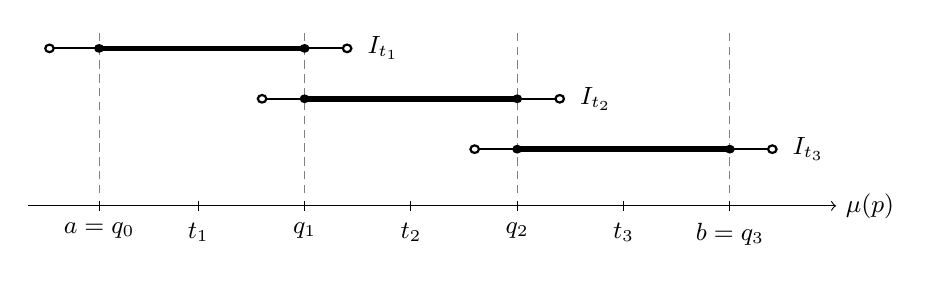
\begin{tikzpicture}[x=0.9cm,y=0.8cm,font=\small]
  \draw[->,thin] (-0.4,0) -- (11.0,0) node[right] {$\mu(p)$};
  \foreach \x/\label in {0.6/{a=q_0},2/{t_1},3.5/{q_1},5/{t_2},6.5/{q_2},8/{t_3},9.5/{b=q_3}} {
    \draw (\x,0.08) -- (\x,-0.08);
    \node[below] at (\x,-0.12) {$\label$};
  }
  \foreach \x in {0.6,3.5,6.5,9.5} {
    \draw[gray,densely dashed,thin] (\x,0.2) -- (\x,2.75);
  }
  \draw[thick] (-0.1,2.5) -- (4.1,2.5);
  \draw[fill=white,thick] (-0.1,2.5) circle (0.06);
  \draw[fill=white,thick] (4.1,2.5) circle (0.06);
  \draw[line width=2pt] (0.6,2.5) -- (3.5,2.5);
  \fill (0.6,2.5) circle (0.07);
  \fill (3.5,2.5) circle (0.07);
  \node[right] at (4.25,2.5) {$I_{t_1}$};
  \draw[thick] (2.9,1.7) -- (7.1,1.7);
  \draw[fill=white,thick] (2.9,1.7) circle (0.06);
  \draw[fill=white,thick] (7.1,1.7) circle (0.06);
  \draw[line width=2pt] (3.5,1.7) -- (6.5,1.7);
  \fill (3.5,1.7) circle (0.07);
  \fill (6.5,1.7) circle (0.07);
  \node[right] at (7.25,1.7) {$I_{t_2}$};
  \draw[thick] (5.9,0.9) -- (10.1,0.9);
  \draw[fill=white,thick] (5.9,0.9) circle (0.06);
  \draw[fill=white,thick] (10.1,0.9) circle (0.06);
  \draw[line width=2pt] (6.5,0.9) -- (9.5,0.9);
  \fill (6.5,0.9) circle (0.07);
  \fill (9.5,0.9) circle (0.07);
  \node[right] at (10.25,0.9) {$I_{t_3}$};
\end{tikzpicture}
\caption{Combining three local families, schematically. Each thick closed
interval $[q_{j-1},q_j]$ lies inside the open neighborhood $I_{t_j}$
where its family is valid. The shifts in \eqref{eq:affine-shifts} force
the limiting minimum exponent of an active label into this closed
interval. At a cut, either neighboring family remains valid.}
\label{fig:intervals}
\end{figure}


Suppose a fixed label from $\Lambda_{t_j}$ is active in the combined
family along $h_\nu\to0+$ and $p^\nu\to p\in[a,b]^m$. Write
$c(h)$ for its original local offset and $h=h_\nu$. We claim
\[
 q_{j-1}\leq\mu(p)\leq q_j.
\]
If $j<N$ and $\mu(p)>q_j$, each coordinate $h^{p_i^\nu}$ is
$o(h^{q_j})$. Also $c(h)=o(h^{q_j})$, by
\eqref{eq:local-decay} and $q_j<R_j=t_j+\rho_{t_j}$. Subtracting
the value of the shifted label $(t_{j+1}\one,0)$ from the active
label's value gives
\[
 (r-t_{j+1}\one)\cdot X_h(p^\nu)+c(h)+h^{q_j}
   =h^{q_j}+o(h^{q_j})>0,
\]
a contradiction.

If $j>1$ and $\mu(p)<q_{j-1}$, compare instead with the shifted
label $(t_{j-1}\one,0)$. The difference is
\[
 (r-t_{j-1}\one)\cdot X_h(p^\nu)+c(h)-h^{q_{j-1}}.
\]
Every coefficient in the scalar product is at least
$t_j-t_{j-1}>0$. Some coordinate has $p_i<q_{j-1}$, so its
exponential divided by $h^{q_{j-1}}$ tends to infinity. Meanwhile,
$c(h)=o(h^{q_{j-1}})$ because $q_{j-1}<t_j<t_j+\rho_{t_j}$.
Thus the displayed difference divided by $h^{q_{j-1}}$ tends to
$+\infty$, again contradicting activity. The outer bounds for $j=1$
or $j=N$ follow from $\mu(p)\in[a,b]$.

By \eqref{eq:affine-cuts}, the claimed bounds place $\mu(p)$ inside
$I_{t_j}$, including when it equals a cut. The label is active within
its original local family, so the guarantee on $I_{t_j}$ gives
$\norm{p-r}_\infty<E(r)$. This completes the induction.
\end{proof}

The sequential formulation yields the uniform statement needed below.
Its order of choices is important: the family, and hence its finite set
of slopes, is fixed before the upper bound on $h$ is chosen.

\begin{corollary}[Uniform activity bound]
\label{cor:activity}
Let $m\geq1$, $a<b$, and $E:[a,b]^m\to(0,\infty)$ be as in
Lemma~\ref{lem:affine}. Fix a family $\Lambda$ supplied by that
lemma. There is $h_0\in(0,1)$ such that, for every $0<h<h_0$ and
every $p\in[a,b]^m$, each label $\lambda\in\Lambda$ active at
$X_h(p)$ satisfies
\[
 \norm{p-r_\lambda}_\infty<E(r_\lambda).
\]
\end{corollary}

\begin{proof}
Otherwise there are $h_\nu\to0+$, points $p^\nu\in[a,b]^m$, and
active labels $\lambda_\nu$ such that
$\norm{p^\nu-r_{\lambda_\nu}}_\infty\geq E(r_{\lambda_\nu})$.
By finiteness and compactness, pass to a subsequence on which
$\lambda_\nu=\lambda$ is fixed and $p^\nu\to p\in[a,b]^m$.
The inequality passes to the limit and contradicts
Lemma~\ref{lem:affine}. No continuity of $E$ is needed because its
argument $r_\lambda$ is fixed on this subsequence.
\end{proof}

\section{Compact plateaux and strict increase}\label{sec:trapping}

We now apply Corollary~\ref{cor:activity} to the reaction network.  For each
sufficiently small scale we will construct a compact set in the positive
orthant that is forward invariant.  For a fixed positive stoichiometric
class, we will also prove that a trajectory in that class remaining in
the scale's box reaches this set in finite time.  The affine
minimum and sign argument adapt the trapping construction of
\cite[Section~3]{OpenAI2026}; the strict increase away from a plateau is the
additional property needed for finite entry within a fixed class.

Use $X_h$ from Section~\ref{sec:affine} with $m=d$, and for $0<h<1$ put
\[
 B_h=[h,h^{-1}]^d.
\]
Every $x\in B_h$ is uniquely $X_h(p)$ for $p\in[-1,1]^d$, with
$p=\log x/\log h$, where the logarithm of a vector is taken coordinatewise.
We first choose the tolerance in Corollary~\ref{cor:activity} so that active
slopes determine both coordinate signs and the ordering of monomials.
Let
\begin{equation}\label{eq:comparison-directions}
 D=\{e_i:1\leq i\leq d\}
   \cup\{z-y:y,z\in C,\ z\ne y\},
\end{equation}
where $e_i$ is the $i$th coordinate vector.  This is a finite set of nonzero
vectors.  We include all pairs of complexes because the flux estimate
will compare sources of different reactions, possibly in different
components of the reaction graph.  Define, for $r\in[-1,1]^d$,
\begin{equation}\label{eq:network-tolerance}
 E(r)=\min\left(
 \left\{\frac12\right\}\cup
 \left\{\frac{\abs{r\cdot v}}{2\norm{v}_1}:
                 v\in D,\ r\cdot v\ne0\right\}\right).
\end{equation}
Zero scalar products impose no sign restriction and are omitted.
Thus $E$ is positive at every point, including on the comparison
hyperplanes; no continuity is needed.
Fix the finite nonempty family supplied by
Corollary~\ref{cor:activity} for this $E$, and write its affine functions as
\[
 L_{\lambda,h}(x)=r_\lambda\cdot x+b_\lambda(h),
 \qquad
 F_h(x)=\min_{\lambda\in\Lambda}L_{\lambda,h}(x).
\]
The slopes $r_\lambda\in[-1,1]^d$ and the index set $\Lambda$ are fixed
independently of $h$.  A label $\lambda$ is active at $x$ if
$L_{\lambda,h}(x)=F_h(x)$; denote the set of these labels by $A_h(x)$.
For every sufficiently small $h$, the activity estimate is
\begin{equation}\label{eq:network-activity}
 x=X_h(p)\in B_h,\quad \lambda\in A_h(x)
 \quad\Longrightarrow\quad
 \norm{p-r_\lambda}_\infty<E(r_\lambda).
\end{equation}

Because the family of slopes is fixed and finite, the number
\begin{equation}\label{eq:uniform-sign-gap}
 H=\min\left(
 \{1\}\cup
 \left\{\frac{\abs{r_\lambda\cdot v}}2:
       \lambda\in\Lambda,\ v\in D,\ r_\lambda\cdot v\ne0\right\}\right)
\end{equation}
is positive.  If $x=X_h(p)\in B_h$, $\lambda\in A_h(x)$, and
$r=r_\lambda$, then
\[
 \abs{(p-r)\cdot v}
 \leq\norm{p-r}_\infty\norm{v}_1
 <E(r)\norm{v}_1
 \leq\frac{\abs{r\cdot v}}2
 \qquad (v\in D,\ r\cdot v\ne0).
\]
Consequently,
\begin{equation}\label{eq:sign-and-size}
 r\cdot v\ne0
 \quad\Longrightarrow\quad
 \operatorname{sgn}(p\cdot v)=\operatorname{sgn}(r\cdot v),
 \qquad \abs{p\cdot v}\geq H
 \qquad (v\in D).
\end{equation}

Fix a positive stoichiometric class $P$, and choose one representative
$c\in P$ once for this class.  Choose $h_P\in(0,1)$ so small that the
affine functions are defined and \eqref{eq:network-activity} holds for
every $0<h\leq h_P$, and also
\begin{equation}\label{eq:class-scale}
 \norm{\frac{\log c}{\log h}}_\infty<H,
 \qquad
 h^H\sum_{e\in R}k_e<\min_{e\in R}k_e
 \quad (0<h\leq h_P).
\end{equation}
The second inequality is imposed only when $R\ne\varnothing$.
Such a choice exists because $H>0$, all the rates are positive, and
both $1/\abs{\log h}$ and $h^H$ tend to zero as $h$ tends to zero.
In particular, $c\in\operatorname{int}B_h$ for these scales.
All the remaining statements of this section concern $0<h\leq h_P$.

\begin{proposition}[The compact plateau]\label{prop:plateau}
For $0<h\leq h_P$, let
\[
 M_h=F_h(c),
 \qquad
 K_h=\{x\in\R^d:F_h(x)=M_h\}.
\]
There is a constant label with value $M_h$, and $F_h\leq M_h$ on
$\R^d$.  The set $K_h$ is nonempty, compact, and convex, and
\begin{equation}\label{eq:plateau-containment}
 K_h\subset\operatorname{int}B_{\sqrt h}.
\end{equation}
\end{proposition}

\begin{proof}
Write $p_c=\log c/\log h$.  If a label active at $c$ had a nonzero
coordinate $r_{\lambda,i}$, \eqref{eq:sign-and-size} with $v=e_i$ would
give $\abs{p_{c,i}}\geq H$, contrary to \eqref{eq:class-scale}.
Thus every label active at $c$ has zero slope.  At least one label is
active there, so one of the affine functions is the constant $M_h$.
It follows that $F_h\leq M_h$ everywhere, and that $M_h$ is the least
value of any constant label.  Hence
\[
 K_h=\bigcap_{\lambda\in\Lambda}
       \{x\in\R^d:L_{\lambda,h}(x)\geq M_h\}
\]
is closed and convex, and contains $c$.

If $x=X_h(p)\in K_h\cap B_h$, the constant label with value $M_h$ is
active at $x$.  Applying \eqref{eq:network-activity} to its zero slope
gives
\[
 \norm{p}_\infty<E(0)=\frac12,
 \qquad\text{and thus}\qquad
 x\in\operatorname{int}B_{\sqrt h}.
\]
In particular, $K_h$ misses the boundary of $B_h$.  If some point of
$K_h$ lay outside $B_h$, the segment joining it to
$c\in\operatorname{int}B_h$ would meet that boundary at a point of
$K_h$, by convexity.  This is impossible.  Thus $K_h\subset B_h$, and
the preceding argument proves \eqref{eq:plateau-containment} for every
point of $K_h$.  Closedness and boundedness give compactness.
\end{proof}

The plateau is now a compact candidate for a trapping set. A slope in
$S^\perp$ gives an affine function that is constant on $P$. We first
exclude such slopes below the plateau, then compare reaction fluxes to
prove strict increase for every remaining active label.

\begin{proposition}[Increase of active affine functions]\label{prop:increase}
Fix $0<h\leq h_P$.  For every $x\in B_h$ and every
$\lambda\in A_h(x)$,
\begin{equation}\label{eq:active-flux-sign}
 r_\lambda\cdot f(x)\geq0,
 \qquad
 r_\lambda\cdot f(x)>0\quad\text{if }r_\lambda\notin S^\perp.
\end{equation}
Moreover, there is a number $\delta_h>0$ such that
\begin{equation}\label{eq:uniform-active-increase}
 r_\lambda\cdot f(x)\geq\delta_h
 \quad\text{whenever }x\in B_h,\ \lambda\in A_h(x),
                       \ r_\lambda\notin S^\perp.
\end{equation}
At every point of $P\setminus K_h$, all active slopes lie outside
$S^\perp$.  In particular, \eqref{eq:uniform-active-increase} applies
to every active label at each $x\in B_h\cap(P\setminus K_h)$.
\end{proposition}

\begin{proof}
First, let $x\in P\setminus K_h$.  If $r_\lambda\in S^\perp$,
then $x-c\in S$ implies
\[
 L_{\lambda,h}(x)=L_{\lambda,h}(c)\geq F_h(c)=M_h.
\]
But $F_h(x)<M_h$ by Proposition~\ref{prop:plateau}.  Such a label
cannot be active at $x$.

If $R$ is empty, then $f=0$ and $S=\{0\}$, so
\eqref{eq:active-flux-sign} holds and
\eqref{eq:uniform-active-increase} is vacuous.  For the flux comparison,
assume $R\ne\varnothing$ and fix $x=X_h(p)\in B_h$ and an active slope $r$.
Whenever $y,z\in C$ satisfy $r\cdot y<r\cdot z$,
\eqref{eq:sign-and-size} applied to $z-y$ gives
\begin{equation}\label{eq:monomial-order}
 \frac{x^z}{x^y}=h^{p\cdot(z-y)}\leq h^H.
\end{equation}
List the distinct values of $r\cdot y$, for $y\in C$, as
$a_1<\cdots<a_m$.  For $1\leq j<m$, define the net upward flux across
the cut at $a_j$ by
\begin{align*}
 Q_j(x)={}&
 \sum_{\substack{u\to u'\in R\,:\\r\cdot u\leq a_j<r\cdot u'}}
       k_{u\to u'}x^u
 -\sum_{\substack{u\to u'\in R\,:\\r\cdot u'\leq a_j<r\cdot u}}
       k_{u\to u'}x^u.
\end{align*}
An edge crossing the cut in the first sum is called upward, and an
edge in the second sum is called downward.

If there is a downward edge $u\to u'$, weak reversibility supplies a
directed path from $u'$ back to $u$.  This path starts below the cut
and ends above it, so it contains an upward edge, say $w\to w'$.
Every source $u$ of a downward edge has $r\cdot u>r\cdot w$.
By \eqref{eq:monomial-order} and \eqref{eq:class-scale},
\[
 \sum_{\substack{u\to u'\in R\,:\\r\cdot u'\leq a_j<r\cdot u}}
       k_{u\to u'}x^u
 \leq h^H x^w\sum_{e\in R}k_e
 < k_{w\to w'}x^w.
\]
Thus one upward edge already contributes more than the entire
downward sum, and $Q_j(x)>0$.  If there is no downward edge, then
$Q_j(x)\geq0$, with strict inequality whenever there is an upward
edge.  In all cases $Q_j(x)$ is nonnegative, and it is positive if
any reaction crosses the cut.

The contribution of an edge to $r\cdot f(x)$ is its flux multiplied
by the difference between the levels of its target and source.
Writing this difference as the signed sum of the intervening gaps gives
\begin{equation}\label{eq:cut-flux-decomposition}
 r\cdot f(x)=\sum_{j=1}^{m-1}(a_{j+1}-a_j)Q_j(x).
\end{equation}
Every term is nonnegative.  If $r\notin S^\perp$, some reaction
$y\to y'$ satisfies $r\cdot(y'-y)\ne0$ and therefore crosses at least
one cut; the corresponding term is positive.  This proves
\eqref{eq:active-flux-sign}.  When $m=1$, the sum is empty and every
reaction has zero scalar product with $r$, as required.  Self-loops
never cross a cut and contribute zero to the vector field.

For the uniform bound, the active set of a fixed label,
\[
 T_{\lambda,h}=
 \{x\in B_h:L_{\lambda,h}(x)=F_h(x)\},
\]
is compact.  If $r_\lambda\notin S^\perp$ and $T_{\lambda,h}$ is
nonempty, the continuous function $r_\lambda\cdot f$ is strictly
positive on this set and has a positive minimum there.  Take the
minimum of these positive numbers over the finitely many eligible
labels.  If there are none, choose any $\delta_h>0$.  This proves
\eqref{eq:uniform-active-increase}, including the case $R=\varnothing$.
\end{proof}

The strict inequality in Proposition~\ref{prop:increase} is uniform at
a fixed scale even near the plateau.  Together with the finite nature
of the affine minimum, this gives a direct finite-time trapping
statement.

\begin{lemma}[Trapping and finite entry]\label{lem:trapping}
Fix $0<h\leq h_P$.  Along any solution segment contained in $B_h$,
the function $t\mapsto F_h(x(t))$ is nondecreasing.  If the segment
$x([s,t])$ is contained in $B_h\cap(P\setminus K_h)$, then
\begin{equation}\label{eq:trajectory-increase}
 F_h(x(t))-F_h(x(s))\geq\delta_h(t-s).
\end{equation}
Every solution starting in $K_h$ exists for all nonnegative time and
remains in $K_h$.  In particular, solutions starting in $K_h\cap P$
remain in $K_h\cap P$.  Finally, any global solution in $P$ that stays
in $B_h$ from some time onward enters $K_h$ in finite time and then
remains there.
\end{lemma}

\begin{proof}
For a solution $x(t)$ and each fixed time $t$ before its maximal
existence time, the right derivative of its affine minimum is
\begin{equation}\label{eq:right-derivative}
 \frac{d^+}{dt}F_h(x(t))
   =\min_{\lambda\in A_h(x(t))}r_\lambda\cdot f(x(t)).
\end{equation}
Indeed, all inactive labels have a positive gap above the minimum at
time $t$.  There are finitely many of them, so continuity excludes
them from the minimum for a sufficiently short time to the right.
For each active label, differentiability of the solution gives
\[
 L_{\lambda,h}(x(t+s))
 =F_h(x(t))+s\,r_\lambda\cdot f(x(t))+o(s)
 \qquad(s\downarrow0).
\]
Taking the minimum of these finitely many expansions proves
\eqref{eq:right-derivative}.

We use the elementary fact that a continuous function $g$ on
$[a,b]$ with right derivative at least $q$ at every point of $[a,b)$
satisfies $g(b)-g(a)\geq q(b-a)$.  For completeness, for any
$\eta>0$ the function $g(u)-qu+\eta u$ has positive right derivative
before $b$.  Its maximum on the compact interval therefore cannot
occur before $b$.  Comparing its values at $a$ and $b$ and then
letting $\eta\downarrow0$ proves the assertion.  Formula
\eqref{eq:right-derivative} and Proposition~\ref{prop:increase} now
give monotonicity in $B_h$, and give \eqref{eq:trajectory-increase}
when the segment lies in $P\setminus K_h$.

Suppose next that $x(0)\in K_h$, and consider the maximal solution of
the polynomial vector field $f$.  Since
$K_h\subset\operatorname{int}B_h$, the solution initially stays in
$B_h$.  On any interval on which it does so, monotonicity and the
global upper bound $F_h\leq M_h$ force
$F_h(x(t))=M_h$.  Hence it remains in $K_h$.  It cannot have a first
exit from $\operatorname{int}B_h$ within its interval of existence:
continuity would place the exit point in both $K_h$ and the boundary
of $B_h$, contradicting Proposition~\ref{prop:plateau}.
Thus the solution stays in the compact set $K_h$ throughout its
maximal interval.  A solution of a smooth vector field that remains
in a compact subset of its domain extends past any finite endpoint
of its interval of existence.  To see the relevant point here, $f$
is bounded on a neighborhood of $K_h$, so a finite endpoint would
give a limit of $x(t)$ in $K_h$, at which local existence continues
the solution.  The solution is therefore global.  It remains
positive by \eqref{eq:plateau-containment}; moreover, $f(x)\in S$
implies $x(t)-x(0)\in S$, so a solution starting in $P$ stays in $P$.

Finally, let a global solution in $P$ remain in $B_h$ for all
$t\geq t_0$.  If it never enters $K_h$ after $t_0$, then
\eqref{eq:trajectory-increase} gives
\[
 F_h(x(t))\geq F_h(x(t_0))+\delta_h(t-t_0)
 \qquad(t\geq t_0),
\]
contradicting $F_h\leq M_h$ for sufficiently large $t$.
It must enter $K_h$ at a finite time, and the forward invariance just
proved keeps it there.
\end{proof}

\section{A common absorbing set for each class}\label{sec:permanence}

Fix a positive stoichiometric class $P$ and its representative $c$, and
retain the scale $h_P$ and the functions $F_h$ from
Section~\ref{sec:trapping}. Lemma~\ref{lem:trapping} gives invariance
at each scale and finite-time entry whenever a trajectory stays in the
corresponding box. Proposition~\ref{prop:plateau} connects these two
properties through
\begin{equation}\label{eq:scale-containment}
 K_h\subset\operatorname{int}B_{\sqrt h}
 \qquad(0<h\leq h_P).
\end{equation}
We now use this relation to replace an initial-point-dependent trapping
set by one fixed set for $P$.

\begin{proof}[Proof of Theorem~\ref{thm:main}]
Let $x^0\in P$. Since $x^0$ is positive, we may choose
$0<h_0\leq h_P$ so small that
\[
 \norm{\frac{\log x^0}{\log h_0}}_\infty<H,
\]
where the logarithm is componentwise and $H>0$ is the fixed separation
constant from Section~\ref{sec:trapping}. In particular, $x^0\in B_{h_0}$.
The coordinate sign comparisons force every label active at $x^0$ to
have slope zero, just as they did at $c$. An active constant label
must have the least value among all constant labels, namely
$M_{h_0}=F_{h_0}(c)$. Hence
\[
 x^0\in K_{h_0}.
\]
Lemma~\ref{lem:trapping} implies that the solution through $x^0$ is
global, stays positive, and remains in $K_{h_0}$. Since $f(x)\in S$,
it also remains in $P$.

Starting at $h_0$, define
\begin{equation}\label{eq:scale-sequence}
 h_{j+1}=\min\{\sqrt{h_j},h_P\}.
\end{equation}
We claim that for every $j$ there is a finite time $T_j$ such that
$x(t)\in K_{h_j}$ for all $t\geq T_j$. The case $j=0$ holds with
$T_0=0$. Suppose it holds at $j$. Because
$h_{j+1}\leq\sqrt{h_j}$, the boxes satisfy
$B_{\sqrt{h_j}}\subset B_{h_{j+1}}$. Thus
\eqref{eq:scale-containment} yields
\[
 x(t)\in B_{h_{j+1}}\quad(t\geq T_j).
\]
The finite-entry assertion of Lemma~\ref{lem:trapping}, followed by
its invariance assertion, supplies a finite $T_{j+1}\geq T_j$ with
$x(t)\in K_{h_{j+1}}$ for all $t\geq T_{j+1}$. This proves the claim.
The argument uses containment in successive boxes; no nesting of the
sets $K_h$ is assumed.

Repeated square roots of $h_0\in(0,1)$ tend to $1$. Since $h_P<1$,
the capped sequence \eqref{eq:scale-sequence} therefore reaches $h_P$
after finitely many steps. We conclude that every solution through a
point of $P$ enters $K_{h_P}$ in finite time and stays there.

Finally set
\[
 K_P=K_{h_P}\cap(c+S).
\]
This is nonempty because it contains $c$, and it is compact and convex
as the intersection of the compact convex set $K_{h_P}$ with a closed
affine subspace. Since $K_{h_P}$ lies in the positive orthant, $K_P\subset P$.
Both $K_{h_P}$ and the affine subspace $c+S$ are forward invariant, so
$K_P$ is forward invariant. The preceding argument proves its absorbing
property. Moreover, $K_P\subset B_{h_P}$, and therefore
$\eps_P=h_P\in(0,1)$ gives
\[
 \eps_P\leq x_i(t)\leq\eps_P^{-1}
 \quad(1\leq i\leq d)
\]
for all sufficiently large $t$, with the entry time allowed to depend
on $x^0$. The scale $h_P$, and hence these bounds, was fixed before
choosing the initial point.
\end{proof}

\bibliographystyle{amsplain}
\begingroup
\small
\bibliography{references}
\endgroup
\end{document}
